\section{Usability Evaluation Approach}
\label{sec:evaluation-approach}

To evaluate the ART Editor a task-based test modality has been chosen, composed by four different tasks. All the tasks involve the design, through the Editor, of specific experiences; during the experiment the following metrics are collected:
\begin{itemize}
    \item[-]The task completion rate, measure of the effectiveness.
    \item[-]The average time required to complete a task, measure of the efficiency.
\end{itemize}

Satisfaction is then measured by means of quantitative and qualitative data collected at the end of all the tasks; the quantitative measure of satisfaction is guaranteed by the System Usability Score \cite{brooke_sus_1996} (in \autoref{appendix:sus}), while a qualitative indication of satisfaction is given by an open-ended questionnaire (\autoref{appendix:openended}).

The method we chose to perform the Usability Evaluation experiment and collect all the relevant data is the unmoderated remote test, consisting in the execution through an external platform (Loop11\footnote{\url{https://www.loop11.com/}}) of a recorded session in users' browsers in which a textual description precedes each task and an always on-top button (\autoref{fig:loop-11-button}) allows to either read again the instructions, end the task or abandon the test (\autoref{fig:loop-11-popup}).

\begin{figure}[H]
    \begin{subfigure}{\textwidth}
    \centering
    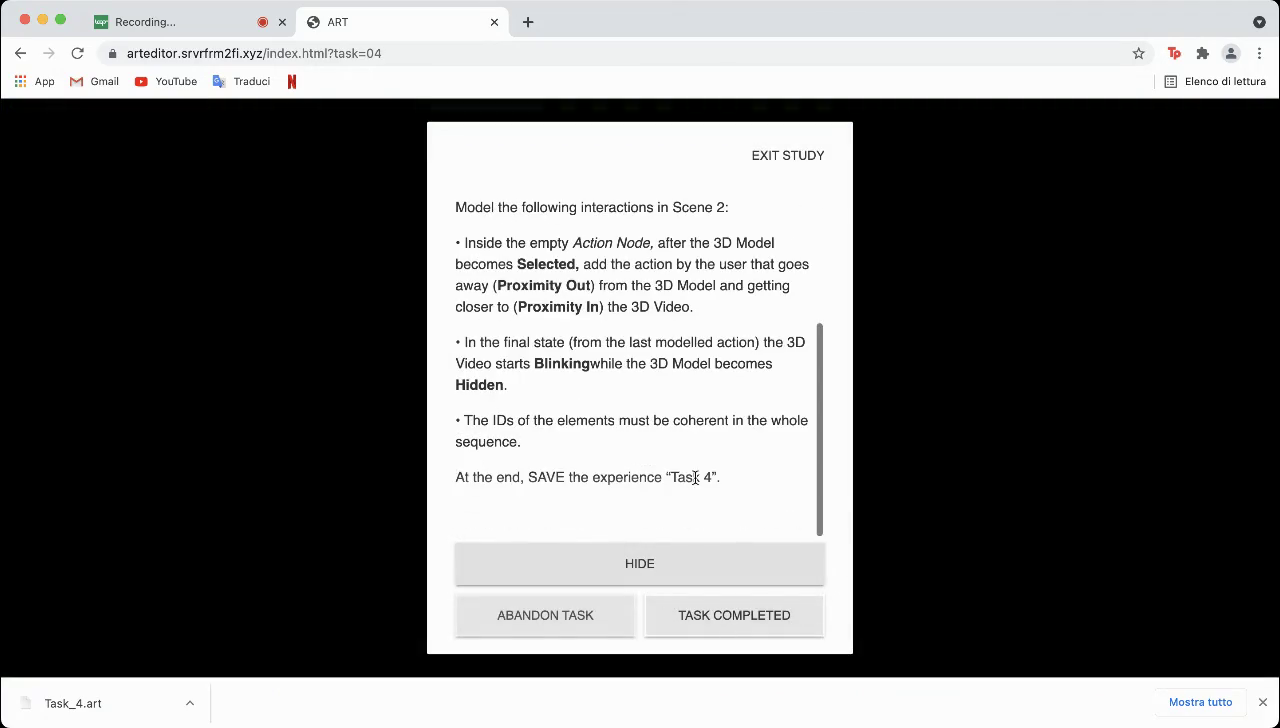
\includegraphics[width=\linewidth]{Figures/Evaluation/eval-platform1.png}
    \caption{}
    \label{fig:loop-11-popup}
    \end{subfigure}
    \begin{subfigure}{\textwidth}
    \centering
    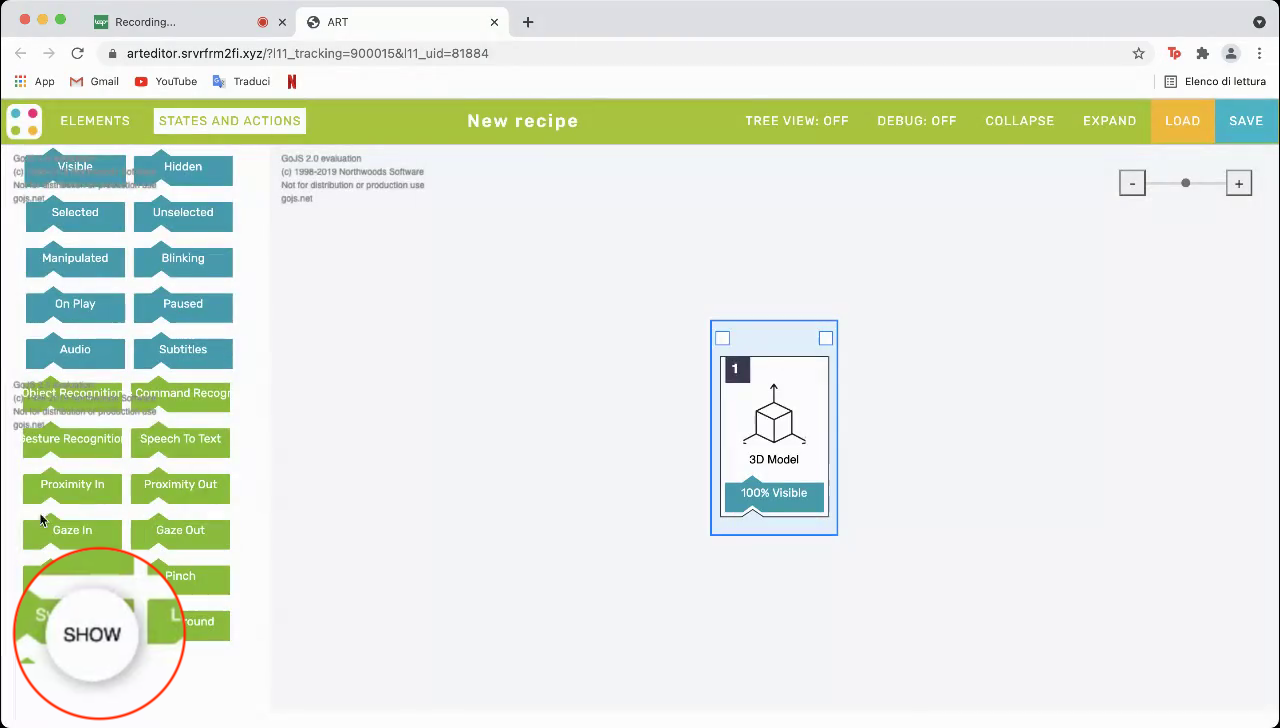
\includegraphics[width=\linewidth]{Figures/Evaluation/eval-platform2.png}
    \caption{}
    \label{fig:loop-11-button}
    \end{subfigure}
\caption{The Loop11 platform executing a test session.}
\label{fig:loop-11}
\end{figure}